\documentclass{beamer}

\usetheme{Singapore}

% Title page details: 
\title{Exercise 11 in Digital Tools for Finance}
\author{S. Kim\inst{1}, M. Kiefer\inst{1}, V. Khmarskyi\inst{1}, B. Clays\inst{2}}
\institute{\inst{1} University of Zürich, \inst{2} KU Leuven}

\begin{document}

\begin{frame}
\titlepage
\end{frame}

\begin{frame}{Title for frame 1}
\framesubtitle{Subtitle for frame 1}

Here is an itemized list of some courses:
\begin{itemize}
    \item Digital Tools for Finance
    \item Financial Engineering
    \item Stress Testing of Banks
\end{itemize}

\bigbreak

Here is an enumeration of some stuff:
\begin{enumerate}
    \item First thing
    \item Second thing
    \item Third thing
\end{enumerate}

\end{frame}
% ---------------------------------------------------------------------------
\begin{frame}{This frame contains a theorem and some math}
\framesubtitle{Both very interesting}

\begin{theorem}
A theorem is a statement that can be demonstrated to be true by accepted mathematical operations and arguments. In general, a theorem is an embodiment of some general principle that makes it part of a larger theory. The process of showing a theorem to be correct is called a proof.\footnotemark
\end{theorem}

\bigbreak

\begin{block}{Unbiased sample variance}
    \begin{equation}
        \sigma_X^2 =\frac{1}{n-1}*\sum_{i=0}^n (X_i-\overline{X})^2
    \end{equation}
\end{block}

\footnotetext[1]{https://mathworld.wolfram.com/Theorem.html}
\end{frame}
% ---------------------------------------------------------------------------
\begin{frame}{Frame 3}
    \framesubtitle{3\textsuperscript{rd} subtitle}

\begin{columns}[T]

    \begin{column}{.5\textwidth}
        \begin{block}{The first panel: Matterhorn}
            
\includegraphics[width=\textwidth]{matterhorn.jpg}
        \end{block}
    \end{column}

    \begin{column}{.5\textwidth}
        \begin{block}{The second panel: a frog}
            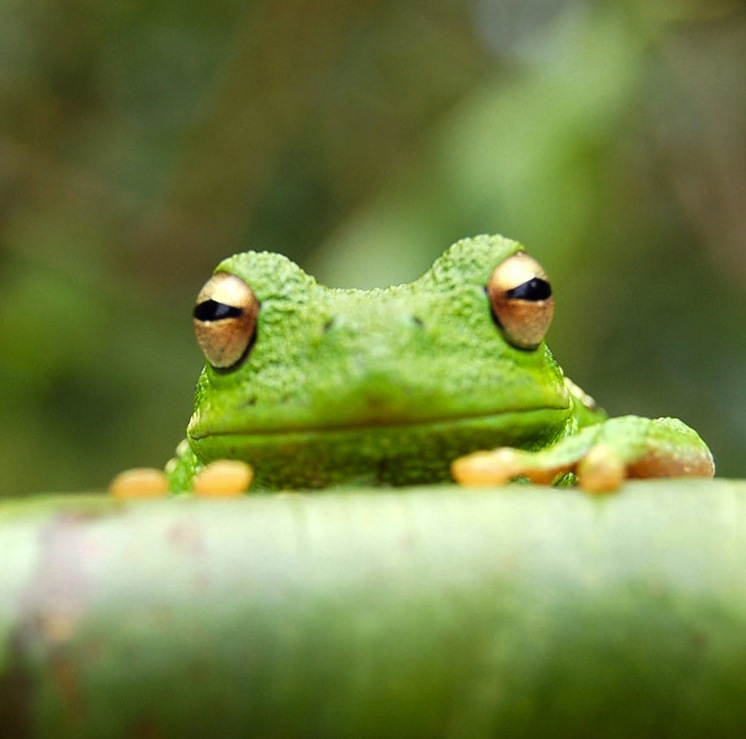
\includegraphics[width=\textwidth]{frog.jpg}
        \end{block}
    \end{column}

\end{columns}   
  
\end{frame}
 
\end{document}